\documentclass[tikz,border=6pt]{standalone}
\usepackage{amsmath,amssymb}
\begin{document}
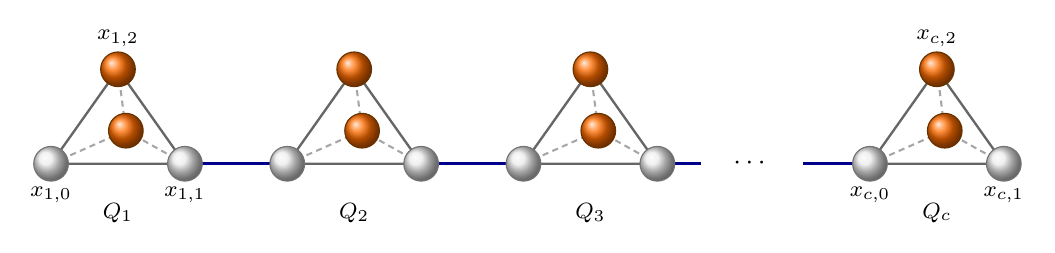
\begin{tikzpicture}[
  v/.style={circle,shading=ball,ball color=white!92!black,draw=black!55,minimum size=4.4mm,inner sep=0pt},
  d/.style={v,ball color=orange!85!red,draw=orange!40!black},
  e/.style={draw=black!60,line width=0.85pt},
  b/.style={draw=black!35,line width=0.75pt,dash pattern=on 2.2pt off 1.6pt},
  br/.style={draw=blue!55!black,line width=1.1pt},
  lab/.style={font=\footnotesize,inner sep=1pt}]
  % one block Q_i: x0 (left), x1 (right), x2 (top), x3 (rear)
  \newcommand{\block}[3]{%
    \coordinate (#1x0) at (#2,0); \coordinate (#1x1) at (#2+1.7,0);
    \coordinate (#1x2) at (#2+0.85,1.2); \coordinate (#1x3) at (#2+0.95,0.42);
    \draw[b] (#1x0)--(#1x3) (#1x1)--(#1x3) (#1x2)--(#1x3);
    \draw[e] (#1x0)--(#1x1)--(#1x2)--(#1x0);
    \node[lab] at (#2+0.85,-0.62) {$#3$};}
  \block{a}{0}{Q_1}
  \block{b}{3.0}{Q_2}
  \block{c}{6.0}{Q_3}
  \block{z}{10.4}{Q_c}
  \draw[br] (ax1)--(bx0); \draw[br] (bx1)--(cx0);
  \draw[br] (cx1)--(8.25,0); \draw[br] (9.55,0)--(zx0);
  \node at (8.9,0) {$\cdots$};
  \foreach \q in {a,b,c,z} {
    \foreach \p in {x0,x1} \node[v] at (\q\p) {};
    \foreach \p in {x2,x3} \node[d] at (\q\p) {};
  }
  \node[lab,below=2.5mm] at (ax0) {$x_{1,0}$}; \node[lab,below=2.5mm] at (ax1) {$x_{1,1}$};
  \node[lab,above=2.5mm] at (ax2) {$x_{1,2}$};
  \node[lab,below=2.5mm] at (zx0) {$x_{c,0}$}; \node[lab,below=2.5mm] at (zx1) {$x_{c,1}$};
  \node[lab,above=2.5mm] at (zx2) {$x_{c,2}$};
\end{tikzpicture}
\end{document}
